\documentclass[a4paper,12pt]{article}
\usepackage[super,square]{natbib}
% Package to change margin size
\usepackage{anysize}
\usepackage{amsmath}
\marginsize{2cm}{2cm}{1cm}{2cm}
% Package to make headers
\usepackage{fancyhdr}
\usepackage{circuitikz}
\renewcommand{\headrulewidth}{0pt}
\usepackage{soul}
\usepackage[section]{placeins}
% Colors for the references links
\usepackage[dvipsnames]{xcolor}
% Package to link references
\usepackage{hyperref}
\usepackage{graphicx}
\usepackage{float}
\hypersetup{
 colorlinks=true,
  linkcolor=black,
  citecolor=CadetBlue,  
  filecolor=CadetBlue,      
  urlcolor=CadetBlue,
}
% Package for lorem ipsum
\usepackage{lipsum}
% Package for multicolumn
\usepackage{multicol}
% Package for removing paragraph identations
\usepackage{parskip}
\setlength\columnsep{18pt}
% Sets bastract
\renewenvironment{abstract}
 {\par\noindent\textbf{\abstractname}\ \ignorespaces \\}
 {\par\noindent\medskip}



 
\begin{document}
% Makes header
\pagestyle{fancy}
\thispagestyle{empty}
\fancyhead[R]{\textit{EE1200}}
\fancyhead[L]{}
% Makes footnotes with an asterisk
\renewcommand*{\thefootnote}{\fnsymbol{footnote}}
\begin{center}
\Large{\textbf{Experiment 05}}
\vspace{0.4cm}
\normalsize
\\ Aditya Tripathy - ee24btech11001, Durgi Swaraj Sharma - ee24btech11018\\
\medskip
\normalsize
\end{center}
{\color{gray}\hrule}
\vspace{0.4cm}
\begin{abstract}
In Experiment-05, we used an Op-amp to make a weighted summing amplifier circuit, an integrator circuit, and a precision rectifier circuit.
\end{abstract}
{\color{gray}\hrule}
\medskip
\section{Part 1 - Custom Weighted summing and difference amplifier}
\subsection{Objective}
To implement the mathematical functions in an inverting amplifier circuit with properly chosen resistors.
\begin{align*}
	V_{out} &= 2V_1+V_2-V_3\\
	V_{out} &= 2V_1-V_3
\end{align*}
\subsection{Apparatus}
\begin{itemize}
	\item Op-amp (we used LM358)
	\item Resistors [$R_1=R$, $R_2=2R$, $R_f=2R$, where we used $R = 10k\Omega$]
	\item Oscilloscope
	\item Two channel function generator
	\item DC power supply	
	\item Connecting wires and probes
\end{itemize}
\subsection{Theory and Circuit}
\begin{figure}[H]
\centering
\resizebox{1\textwidth}{!}{%
\begin{circuitikz}
\tikzstyle{every node}=[font=\normalsize]

\draw (8.5,15.75) node[op amp,scale=1] (opamp2) {};
\draw (opamp2.+) to[short] (7,15.25);
\draw  (opamp2.-) to[short] (7,16.25);
\draw (9.7,15.75) to[short](10,15.75);
\draw (4,16.75) to[R] (5.75,16.75);
\draw (4,16.25) to[R] (5.75,16.25);
\draw (5.75,16.75) to[short] (5.75,16.25);
\draw (5.75,16.25) to[short] (7,16.25);
\node [font=\normalsize] at (4.75,17.25) {$R_1$};
\node [font=\normalsize] at (4.75,15.75) {$R_2$};
\draw (4,15.25) to[R] (6,15.25);
\draw (6,15.25) to[R] (6,13.25);
\draw (6,15.25) to[short] (7,15.25);
\draw (6,13.25) to (8,13.25) node[ground]{};
\draw (6.75,16.25) to[short] (6.75,17.25);
\draw (6.75,17.25) to[R] (9.75,17.25);
\node [font=\normalsize] at (5,14.75) {$R_3$};
\node [font=\normalsize] at (6.5,14.25) {$R_0$};
\draw (9.75,17.25) to[short] (9.75,15.75);
\draw (10,15.75) to[R] (10,13.25);
\draw (10,13.25) to (12,13.25) node[ground]{};
\node [font=\normalsize] at (8,17.75) {$R_f$};
\node [font=\normalsize] at (9.5,14.75) {$R_{out}$};
\end{circuitikz}
}%

\label{fig:my_label}
\end{figure}
A weighted summing amplifier is a circuit that outputs a linear combination of multiple input voltages with different weightings. It is typically implemented using an operational amplifier (op-amp) in the inverting configuration.

An inverting summing amplifier follows the general equation:
\begin{equation}
	V_{out} = - R_f \left( \frac{V_1}{R_1} + \frac{V_2}{R_2} \right) + V_3\frac{R_0}{R_3+R_0}
\end{equation}
where:
\begin{itemize}
    \item $V_1, V_2, V_3$ are the input voltages,
    \item $R_1, R_2$ are the corresponding input resistances,
    \item $R_f$ is the feedback resistance.
    \item $R_0$ is a resistor needed for the circuit to function, not of significance 
\end{itemize}

For the given equations:

\textbf{For the sum \( V_{out} = 2V_1 + V_2 - V_3 \)}\\
To achieve the required weighting, we select:
\begin{equation}
    R_1 = R, \quad R_2 = 2R, \quad R_3 = 0 \quad R_f = 2R.
\end{equation}
Substituting into the summing amplifier equation:
\begin{align*}
    V_{out} &= -2V_1 - V_2 + V_3.
\end{align*}
To correct the sign, we add a second inverting stage to obtain:
\begin{align*}
    V_{out} &= 2V_1 + V_2 - V_3.
\end{align*}
\textbf{For the sum \( V_{out} = 2V_1 - V_3 \)}\\
For this equation, we use:
\begin{equation}
    V_2 = 0,\quad R_1 = R,\quad R_2 = 0,\quad R_3 = 0, \quad R_f = 2R.
\end{equation}
Substituting:
\begin{align*}
    V_{out} &= -2V_1 + V_3.
\end{align*}
Adding an additional inverting stage:
\begin{align*}
    V_{out} &= 2V_1 - V_3.
\end{align*}

\subsection{Procedure}
\begin{enumerate}
	\item IC
		\begin{itemize}
			\item Use the datasheet of your Op-amp to know the function of its pins and specifications.
			\item Ensure the supply voltages $V_+$ and $V_-$ being provided are within the recommended range in the datasheet, before you turn them on (We used $+15V$ and $-15V$).
		\end{itemize}
	\item Circuit
		\begin{itemize}
			\item Make the circuits as shown in the theory section using the right pins of the Op-amp, resistors, and connecting wires.
			\item Use function generator and DC power supply to make the desired $V_1$, $V_2$, and $V_3$.
			\item Apply the voltages and grounds to the circuit to complete it.
		\end{itemize}
	\item Oscilloscope: Use the probe to measure voltage at Op-amp output, i.e. across $R_a$
\end{enumerate}
\subsection{Demonstration}
\begin{figure}[H]
	\centering
	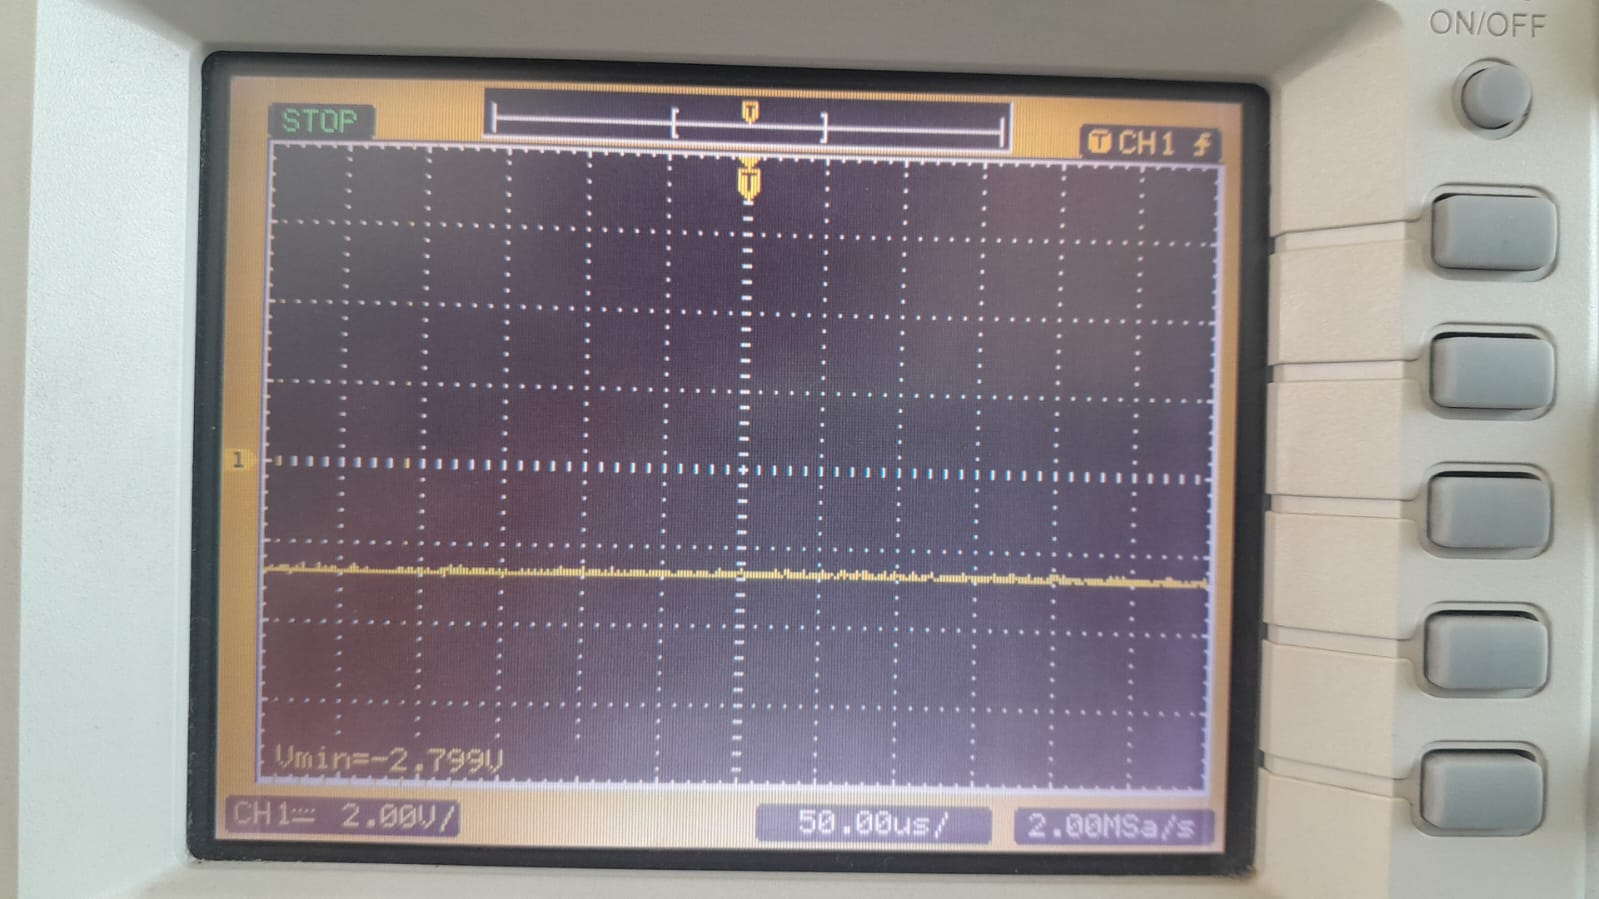
\includegraphics[width = 0.7\columnwidth]{figs/exp1f3.jpg}
	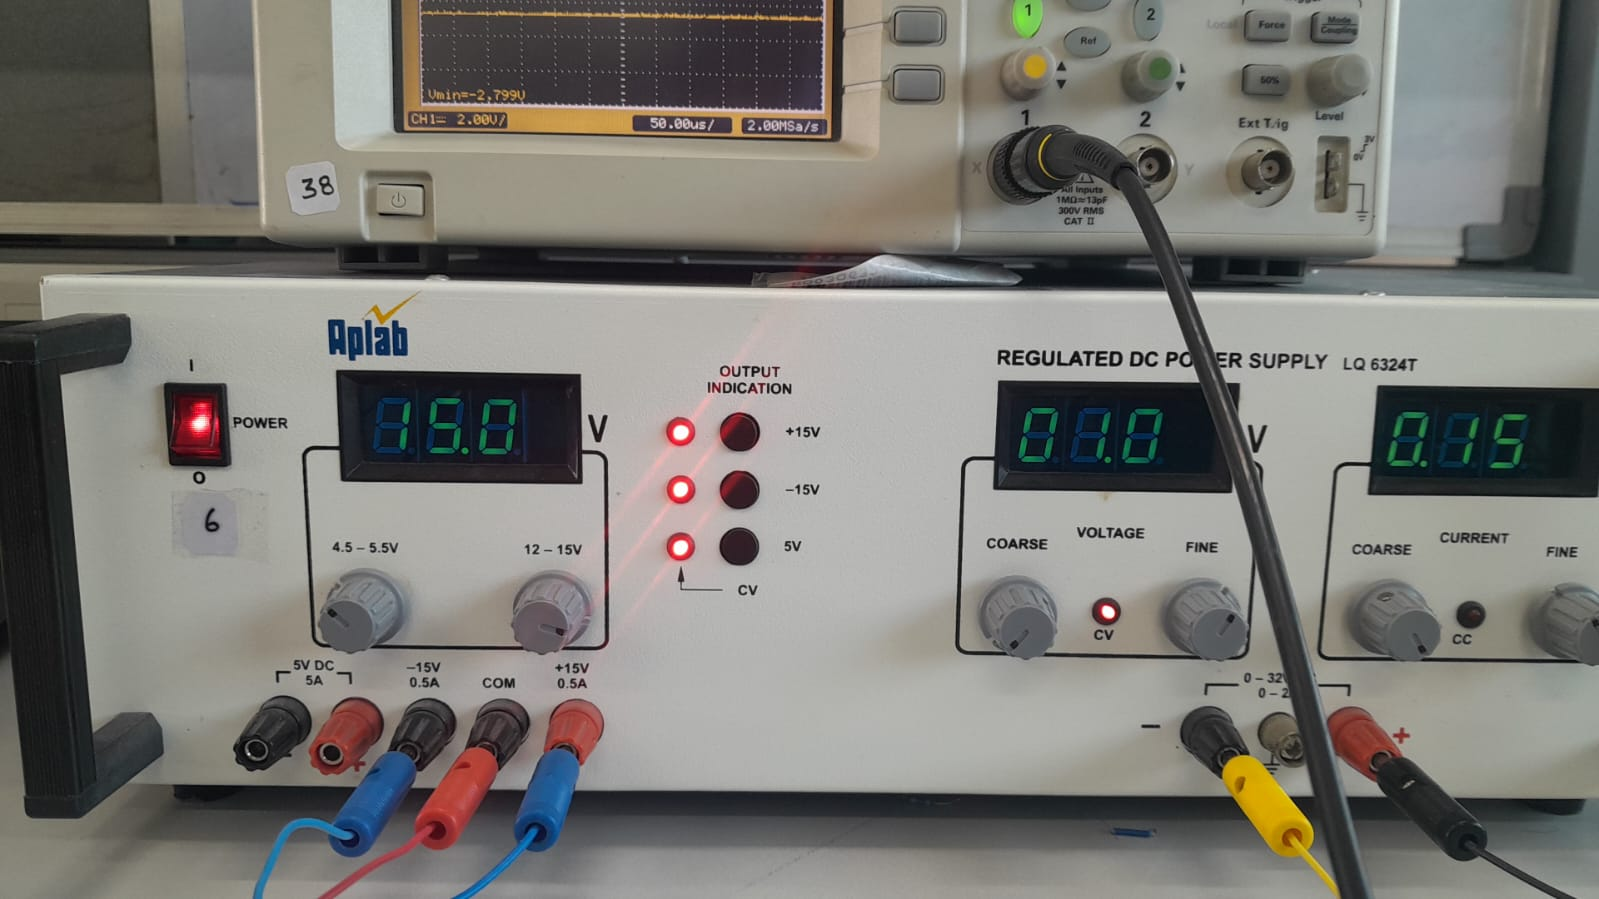
\includegraphics[width = 0.7\columnwidth]{figs/exp1f2.jpg}
	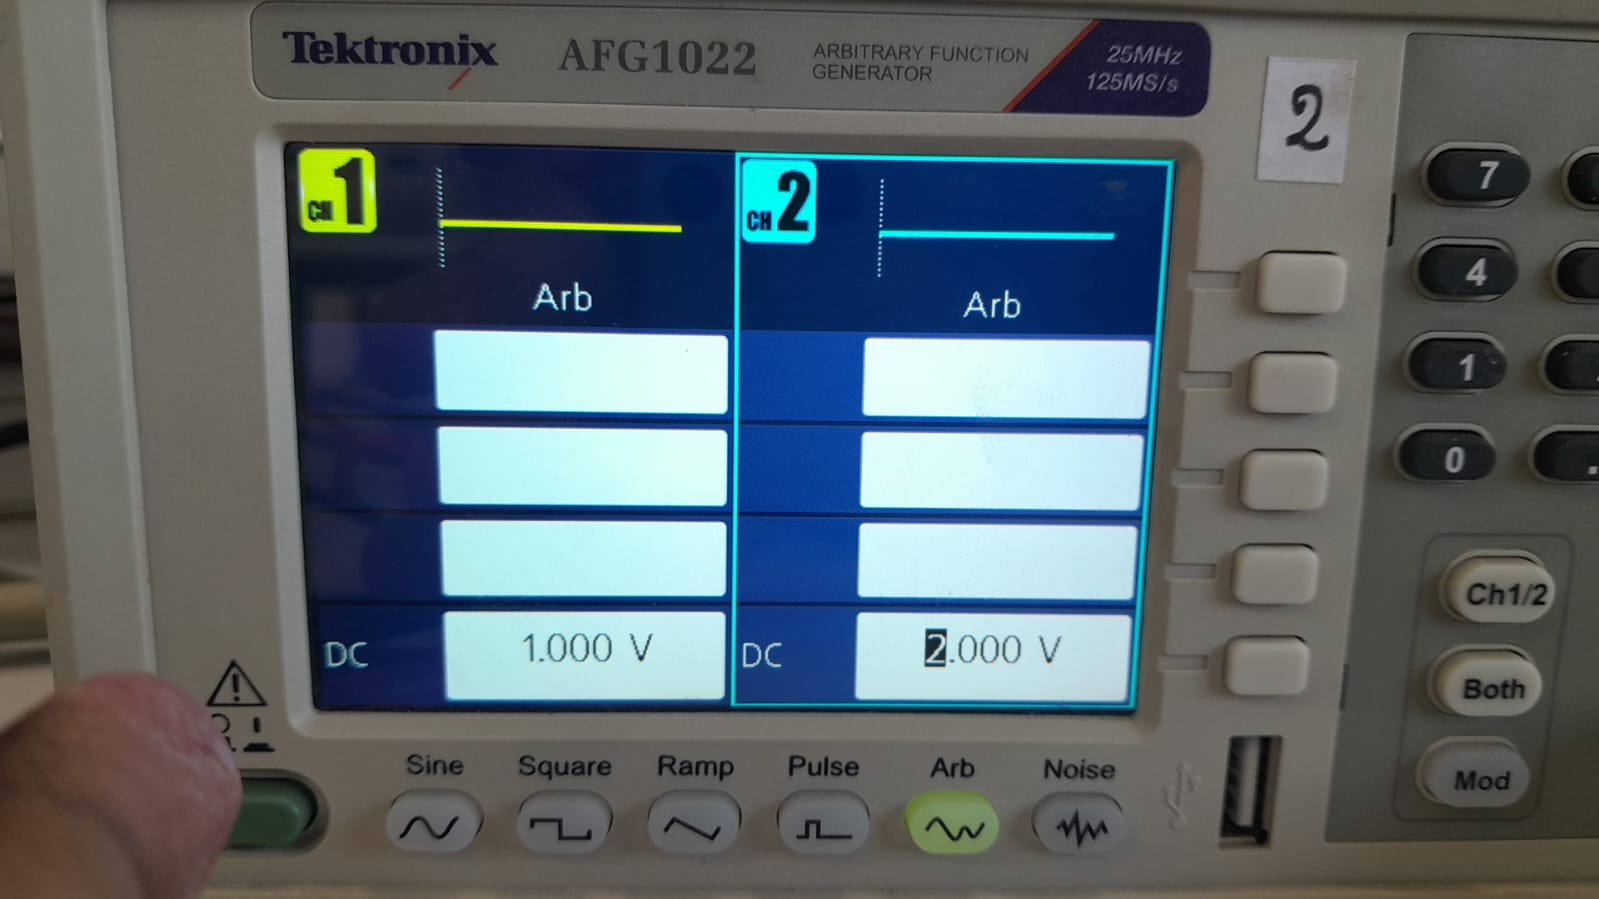
\includegraphics[width = 0.7\columnwidth]{figs/ex1f1.jpg}
	\caption{$2V_1+V_2-V_3$(approximately), $V_1,\,V_2$ on the function generator, $V_3$ from the DC supply(right)}
\end{figure}
\begin{figure}[H]
	\centering
	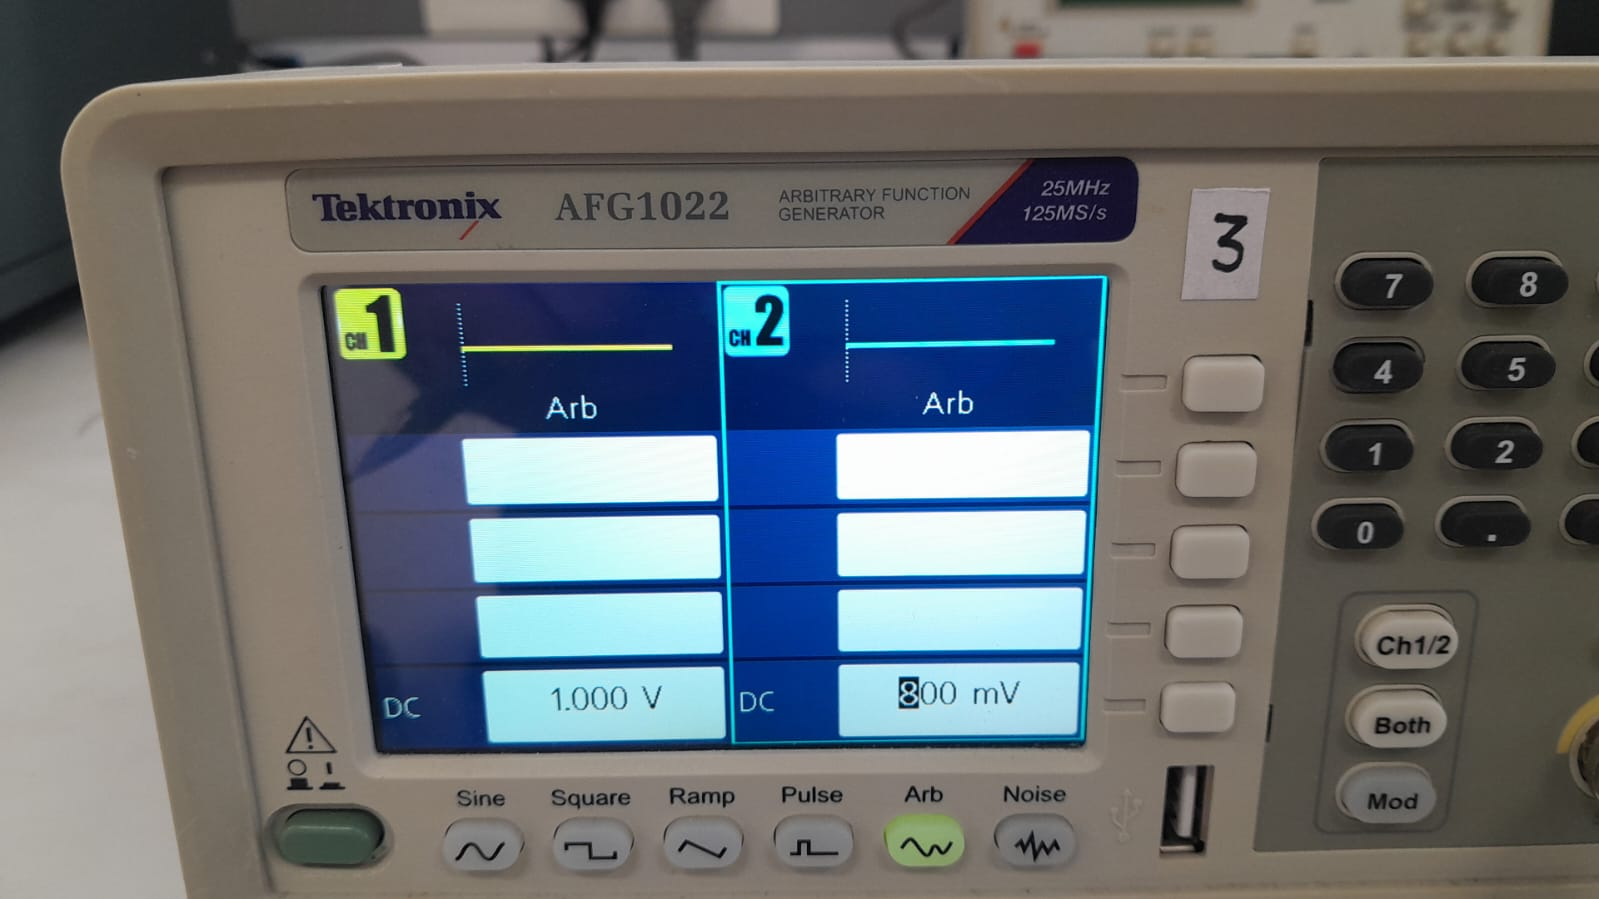
\includegraphics[width = 0.7\columnwidth]{figs/ex1f4.jpg}
	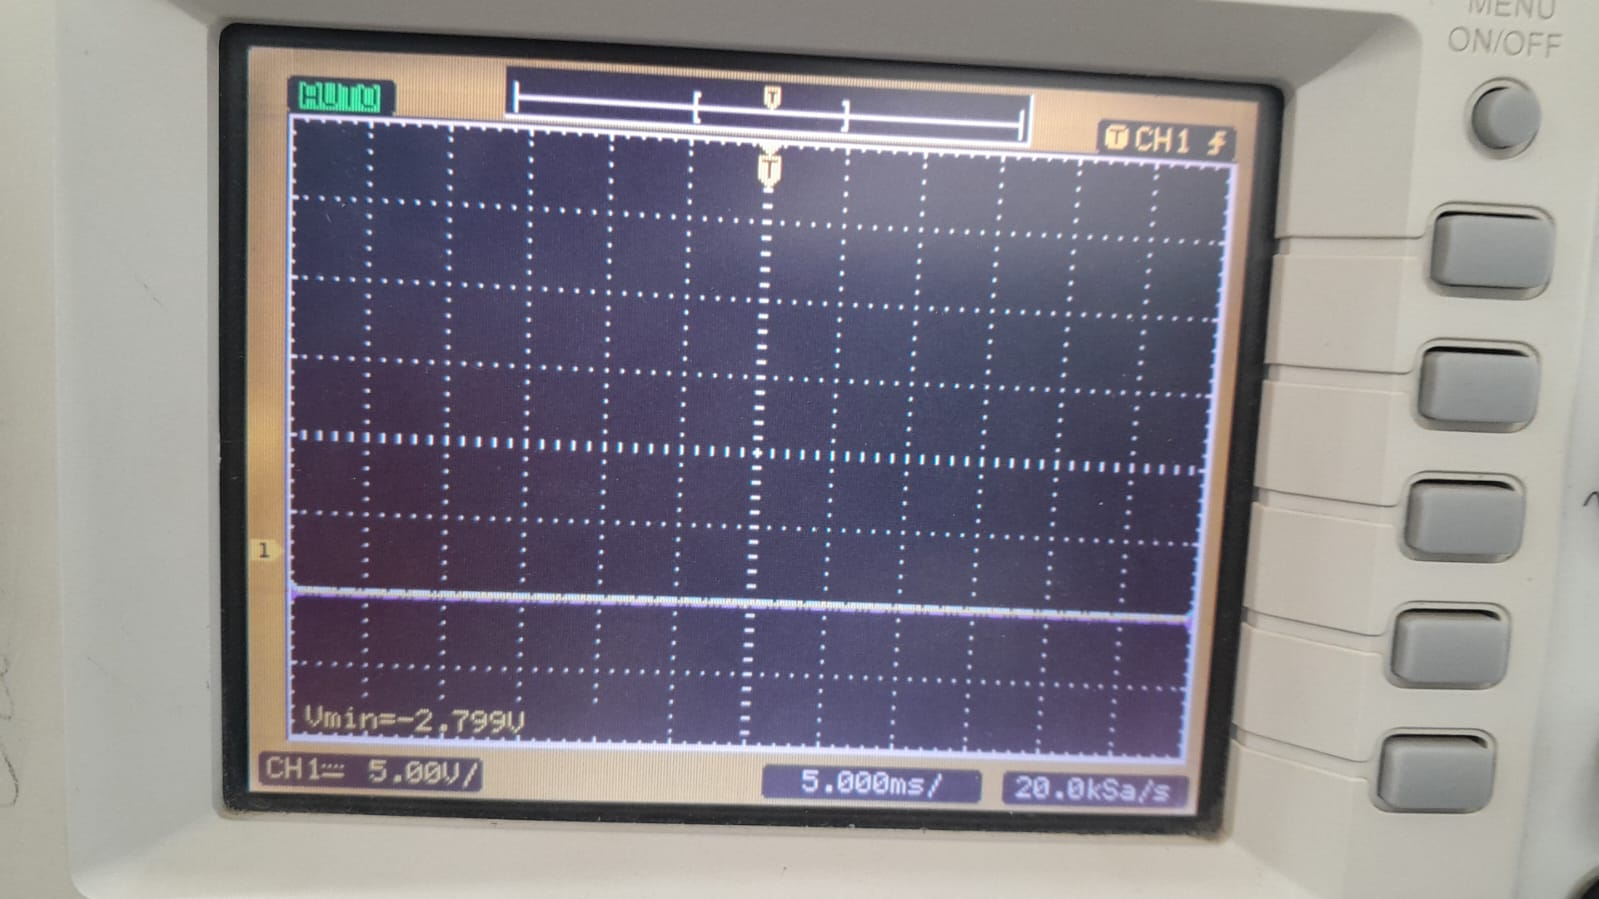
\includegraphics[width = 0.7\columnwidth]{figs/ex4f5.jpg}
	\caption{$2V_1+V_2$, $V_1,\,V_2$ on the function generator}
\end{figure}
\subsection{Conclusion}
We used an Op-amp inverting amplifier to carry out weighted sums of our desired voltages. Our input voltage ranges were limited by the chosen Op-amp compoment, and the circuit would only work if the output volate was within the supply range.
\section{Part 2 - Op-Amp Integrator}

\subsection{Objective}
To design and implement an op-amp integrator circuit that performs mathematical integration of an input voltage signal.

\subsection{Apparatus}
\begin{itemize}
    \item Op-amp (we used LM358)
    \item Resistors \( R \) (value to be determined)
    \item Capacitor \( C \) (value to be determined)
    \item Oscilloscope
    \item Function generator
    \item DC power supply
    \item Connecting wires and probes
\end{itemize}

\subsection{Theory}
An op-amp integrator is a circuit that produces an output proportional to the time integral of the input voltage. It is implemented using an operational amplifier with a capacitor in the feedback path and a resistor at the input.

The general equation for an ideal inverting integrator is:
\begin{equation}
    V_{out} = - \frac{1}{RC} \int V_{in} dt
\end{equation}
where:
\begin{itemize}
    \item \( V_{in} \) is the input voltage,
    \item \( R \) is the input resistance,
    \item \( C \) is the feedback capacitance,
    \item \( V_{out} \) is the integrated output voltage.
\end{itemize}

To design the circuit, we choose appropriate values for \( R \) and \( C \) to achieve the desired time constant \( \tau = RC \).

\begin{figure}[H]
\centering
\resizebox{0.6\textwidth}{!}{%
\begin{circuitikz}
\tikzstyle{every node}=[font=\Large]

\draw (9,9.75) node[op amp,scale=1, yscale=-1 ] (opamp2) {};
\draw (opamp2.+) to[short] (7.5,10.25);
\draw  (opamp2.-) to[short] (7.5,9.25);
\draw (10.2,9.75) to[short](10.5,9.75);
\draw (7.5,11.5) to[C,l={ \Large C}] (10.25,11.5);
\draw (7.5,11.5) to[short] (7.5,10.25);
\draw (10.25,11.5) to[short] (10.25,9.75);
\draw (7.5,10.25) to[R,l={ \Large $R_1$}] (5.75,10.25);
\draw (10.5,9.75) to[R,l={ \Large $R_a$}] (10.5,8);
\draw (7.5,9.25) to (7.5,9) node[ground]{};
\draw (10.5,8.25) to (10.5,8) node[ground]{};
\node [font=\Large] at (5.5,10.25) {$V_{in}$};
\end{circuitikz}
}
	\caption{Op-amp Integrator circuit}
\label{fig:my_label}
\end{figure}

\subsection{Procedure}
\begin{enumerate}
    \item \textbf{IC Setup}
    \begin{itemize}
        \item Refer to the Op-amp datasheet to identify pin functions and electrical characteristics.
        \item Ensure the power supply voltages \( V_+ \) and \( V_- \) are within the recommended range (we used +15V and -15V).
    \end{itemize}
    \item \textbf{Circuit Assembly}
    \begin{itemize}
	    \item Connect the circuit as shown in the diagram using appropriate resistor \( R \) and capacitor \( C \) values (we used $R=1\mu F$ and $C=10k\Omega$).
        \item Apply a known input signal \( V_{in} \) using a function generator (e.g., a square wave).
        \item Connect the oscilloscope to measure \( V_{out} \).
    \end{itemize}
    \item \textbf{Oscilloscope Measurement}
    \begin{itemize}
        \item Observe the output waveform to verify integration behavior.
        \item Compare with the expected theoretical response.
    \end{itemize}
\end{enumerate}

\subsection{Demonstration}
\begin{figure}[H]
	\includegraphics[width=\columnwidth]{figs/integrator.jpg}
\end{figure}
For a square wave input:
\begin{itemize}
    \item Assume a square wave of amplitude \( A \) and period \( T \), given by:
    \begin{equation}
        V_{in}(t) = \begin{cases} A, & 0 \leq t < \frac{T}{2} \\
        -A, & \frac{T}{2} \leq t < T \end{cases}
    \end{equation}
    \item Integrating \( V_{in} \) over time:
    \begin{equation}
        V_{out}(t) = -\frac{1}{RC} \int V_{in}(t) dt
    \end{equation}
    \item For \( 0 \leq t < \frac{T}{2} \):
    \begin{equation}
        V_{out}(t) = -\frac{A}{RC} t + V_{out}(0)
    \end{equation}
    \item For \( \frac{T}{2} \leq t < T \):
    \begin{equation}
        V_{out}(t) = \frac{A}{RC} (t - T/2) + V_{out}(T/2)
    \end{equation}
\end{itemize}
Thus, the output is a triangular wave with a slope of \( \pm A/RC \), confirming that an op-amp integrator converts a square wave input into a triangular wave output.

\subsection{Conclusion}
The op-amp integrator successfully performed mathematical integration, converting an input square wave into a triangular wave. The response was dependent on the values of \( R \) and \( C \), confirming the theoretical integration formula. The circuit functioned correctly within the op-amp's operational limits.
\section{Part 3 - Precision Rectifier}
\subsection{Objective}
To design a wave rectifier with and without using an Op-amp to demonstrate the lack of voltage drop issue in the Precision Rectifier (Op-amp)

\subsection{Apparatus}
\begin{itemize}
\item Op-Amp (LM 358)
\item Two 10$k\Omega$ resistors
\item Two PN - junction diodes
\item Oscilloscope
\item Function Generator
\end{itemize}
\subsection{Theory}

The half wave rectifier implemented with a series connection of a resistor and a PN-junction diode is suboptimal in its working due to the threshold voltage required for the flow of current in the 
positive half cycle of the input wave. 

To implement a better half wave rectifer free from the above mentioned problem we use the following circuit which makes use of an op-amp and a couple of diodes commonly known as a precision half wave
rectifier or a superdiode.

\begin{figure}[!ht]
\centering
\resizebox{0.5\textwidth}{!}{%
\begin{circuitikz}
\tikzstyle{every node}=[font=\normalsize]

\draw (11.5,15.5) node[op amp,scale=1, yscale=-1 ] (opamp2) {};
\draw (opamp2.+) to[short] (10,16);
\draw  (opamp2.-) to[short] (10,15);
\draw (12.7,15.5) to[short](13,15.5);
\draw (10,15) to[R] (7.25,15);
\draw (9.5,15) to[short] (9.5,10.5);
\draw (9.5,12.25) to[D] (13.25,12.25);
\draw (13,15.5) to[D] (16,15.5);
\draw (13.25,12.25) to[short] (13.25,15.5);
\draw (9.5,10.5) to[R] (16,10.5);
\draw (10,16) to (6,16) node[ground]{};
\node [font=\normalsize] at (12.75,10) {$R_f$};
\node [font=\normalsize] at (11.5,11.75) {$D_1$};
\node [font=\normalsize] at (14.5,14.75) {$D_2$};
\node [font=\normalsize] at (8.5,14.5) {$R_1$};
\node [font=\normalsize] at (6.75,15) {V(t)};
\node [font=\normalsize] at (18.75,15.5) {$V_{out}$};
\draw (16,10.5) to[short] (16,15.5);
\draw (16,15.5) to[short] (18.25,15.5);
\node [font=\normalsize] at (13.25,15.75) {$V_o$};
\draw (11.5,15.5) node[op amp,scale=1, yscale=-1 ] (opamp2) {};
\draw (opamp2.+) to[short] (10,16);
\draw  (opamp2.-) to[short] (10,15);
\draw (12.7,15.5) to[short](13,15.5);
\draw (11.5,15.5) node[op amp,scale=1, yscale=-1 ] (opamp2) {};
\draw (opamp2.+) to[short] (10,16);
\draw  (opamp2.-) to[short] (10,15);
\draw (12.7,15.5) to[short](13,15.5);
\draw (11.5,15.5) node[op amp,scale=1, yscale=-1 ] (opamp2) {};
\draw (opamp2.+) to[short] (10,16);
\draw  (opamp2.-) to[short] (10,15);
\draw (12.7,15.5) to[short](13,15.5);
\node [font=\normalsize] at (9.5,15.25) {$V_b$};
\end{circuitikz}
}%

\caption{Precision Rectifier}
\end{figure}

Initially all voltages are at 0V. When $V(t) > 0$, $V_o$ will also become positive. Thus, the flow of current will be as shown:
\begin{figure}[!ht]
\centering
\resizebox{0.5\textwidth}{!}{%
\begin{circuitikz}
\tikzstyle{every node}=[font=\normalsize]

\draw (11.5,15.5) node[op amp,scale=1, yscale=-1 ] (opamp2) {};
\draw (opamp2.+) to[short] (10,16);
\draw  (opamp2.-) to[short] (10,15);
\draw (12.7,15.5) to[short](13,15.5);
\draw (10,15) to[R] (7.25,15);
\draw (9.5,15) to[short] (9.5,10.5);
\draw (9.5,12.25) to[D] (13.25,12.25);
\draw (13,15.5) to[D] (16,15.5);
\draw (13.25,12.25) to[short] (13.25,15.5);
\draw (9.5,10.5) to[R] (16,10.5);
\draw (10,16) to (6,16) node[ground]{};
\node [font=\normalsize] at (12.75,10) {$R_f$};
\node [font=\normalsize] at (11.5,11.75) {$D_1$};
\node [font=\normalsize] at (14.5,14.75) {$R_2$};
\node [font=\normalsize] at (8.5,14.5) {$R_1$};
\node [font=\normalsize] at (6.75,15) {V(t)};
\node [font=\normalsize] at (18.75,15.5) {$V_{out}$};
\draw (16,10.5) to[short] (16,15.5);
\draw (16,15.5) to[short] (18.25,15.5);
\node [font=\normalsize] at (13.25,15.75) {$V_o$};
\draw (11.5,15.5) node[op amp,scale=1, yscale=-1 ] (opamp2) {};
\draw (opamp2.+) to[short] (10,16);
\draw  (opamp2.-) to[short] (10,15);
\draw (12.7,15.5) to[short](13,15.5);
\draw (11.5,15.5) node[op amp,scale=1, yscale=-1 ] (opamp2) {};
\draw (opamp2.+) to[short] (10,16);
\draw  (opamp2.-) to[short] (10,15);
\draw (12.7,15.5) to[short](13,15.5);
\draw (11.5,15.5) node[op amp,scale=1, yscale=-1 ] (opamp2) {};
\draw (opamp2.+) to[short] (10,16);
\draw  (opamp2.-) to[short] (10,15);
\draw (12.7,15.5) to[short](13,15.5);
\draw [->, >=Stealth] (7.5,13.75) -- (9.25,13.75);
\draw [->, >=Stealth] (9,13.25) -- (9,12.25);
\draw [->, >=Stealth] (9.75,12.75) -- (12.5,12.75);
\draw [->, >=Stealth] (13,13.25) -- (13,15);
\draw [->, >=Stealth] (12.5,15) -- (12,15);
\end{circuitikz}
}%
\caption{Current flow for positive half cycle}
\end{figure}
\newline
\newline
\newline
It is evident that the voltage at the $V_{out}$ is zero since the voltages at $t=0$ were all zero. 
\newline
When the input voltage is negative, the flow of current will be as follows:

\begin{figure}[!ht]
\centering
\resizebox{0.5\textwidth}{!}{%
\begin{circuitikz}
\tikzstyle{every node}=[font=\normalsize]

\draw (11.5,15.5) node[op amp,scale=1, yscale=-1 ] (opamp2) {};
\draw (opamp2.+) to[short] (10,16);
\draw  (opamp2.-) to[short] (10,15);
\draw (12.7,15.5) to[short](13,15.5);
\draw (10,15) to[R] (7.25,15);
\draw (9.5,15) to[short] (9.5,10.5);
\draw (9.5,12.25) to[D] (13.25,12.25);
\draw (13,15.5) to[D] (16,15.5);
\draw (13.25,12.25) to[short] (13.25,15.5);
\draw (9.5,10.5) to[R] (16,10.5);
\draw (10,16) to (6,16) node[ground]{};
\node [font=\normalsize] at (12.75,10) {$R_f$};
\node [font=\normalsize] at (11.5,11.75) {$D_1$};
\node [font=\normalsize] at (14.5,14.75) {$D_2$};
\node [font=\normalsize] at (8.5,14.5) {$R_1$};
\node [font=\normalsize] at (6.75,15) {V(t)};
\node [font=\normalsize] at (18.75,15.5) {$V_{out}$};
\draw (16,10.5) to[short] (16,15.5);
\draw (16,15.5) to[short] (18.25,15.5);
\node [font=\normalsize] at (13.25,15.75) {$V_o$};
\draw (11.5,15.5) node[op amp,scale=1, yscale=-1 ] (opamp2) {};
\draw (opamp2.+) to[short] (10,16);
\draw  (opamp2.-) to[short] (10,15);
\draw (12.7,15.5) to[short](13,15.5);
\draw (11.5,15.5) node[op amp,scale=1, yscale=-1 ] (opamp2) {};
\draw (opamp2.+) to[short] (10,16);
\draw  (opamp2.-) to[short] (10,15);
\draw (12.7,15.5) to[short](13,15.5);
\draw (11.5,15.5) node[op amp,scale=1, yscale=-1 ] (opamp2) {};
\draw (opamp2.+) to[short] (10,16);
\draw  (opamp2.-) to[short] (10,15);
\draw (12.7,15.5) to[short](13,15.5);
\draw [->, >=Stealth] (9.25,14) -- (7,14);
\draw [->, >=Stealth] (9,10.75) -- (9,13.75);
\draw [->, >=Stealth] (15.75,11) -- (10,11);
\draw [->, >=Stealth] (11.75,16.25) -- (16,16.25);
\draw [->, >=Stealth] (16.75,15.25) -- (16.75,10.5);
\node [font=\normalsize] at (9.5,15.25) {$V_b$};
\end{circuitikz}
}
\caption{Current flow for negative half cycle}
\end{figure}
The voltage at $V_{out}$ will approximately be equal to
\begin{align}
  V_{out} \approx \frac{-R_f}{R_1}V(t)
\end{align}
\newline
The advantage of the superdiode is that for the current to start flowing, the input voltage need
to be close to ratio of threshold voltage and open loop gain(a very large number)
\begin{align}
  V(t) \approx \frac{V_{th}}{A}, \text{where A = open loop gain}
\end{align}
as opposed to the threshold voltage in the resistor-diode-only approach. Thus a superdiode can be used to rectify signals of amplitude $\approx 100mV$.
\subsection{Procedure}
\begin{enumerate}
\item Connections
\begin{itemize}
\item Connect the circuit as shown in Figure 1.
\item Connect $V_+$ to $15 V$ and $V_-$ to $-15 V$ 
\item Connect the probe of the oscilloscope across the common ground and output pin of the LM358.
\end{itemize}
\end{enumerate}

\subsection{Response captured}
\begin{figure}[H]
  {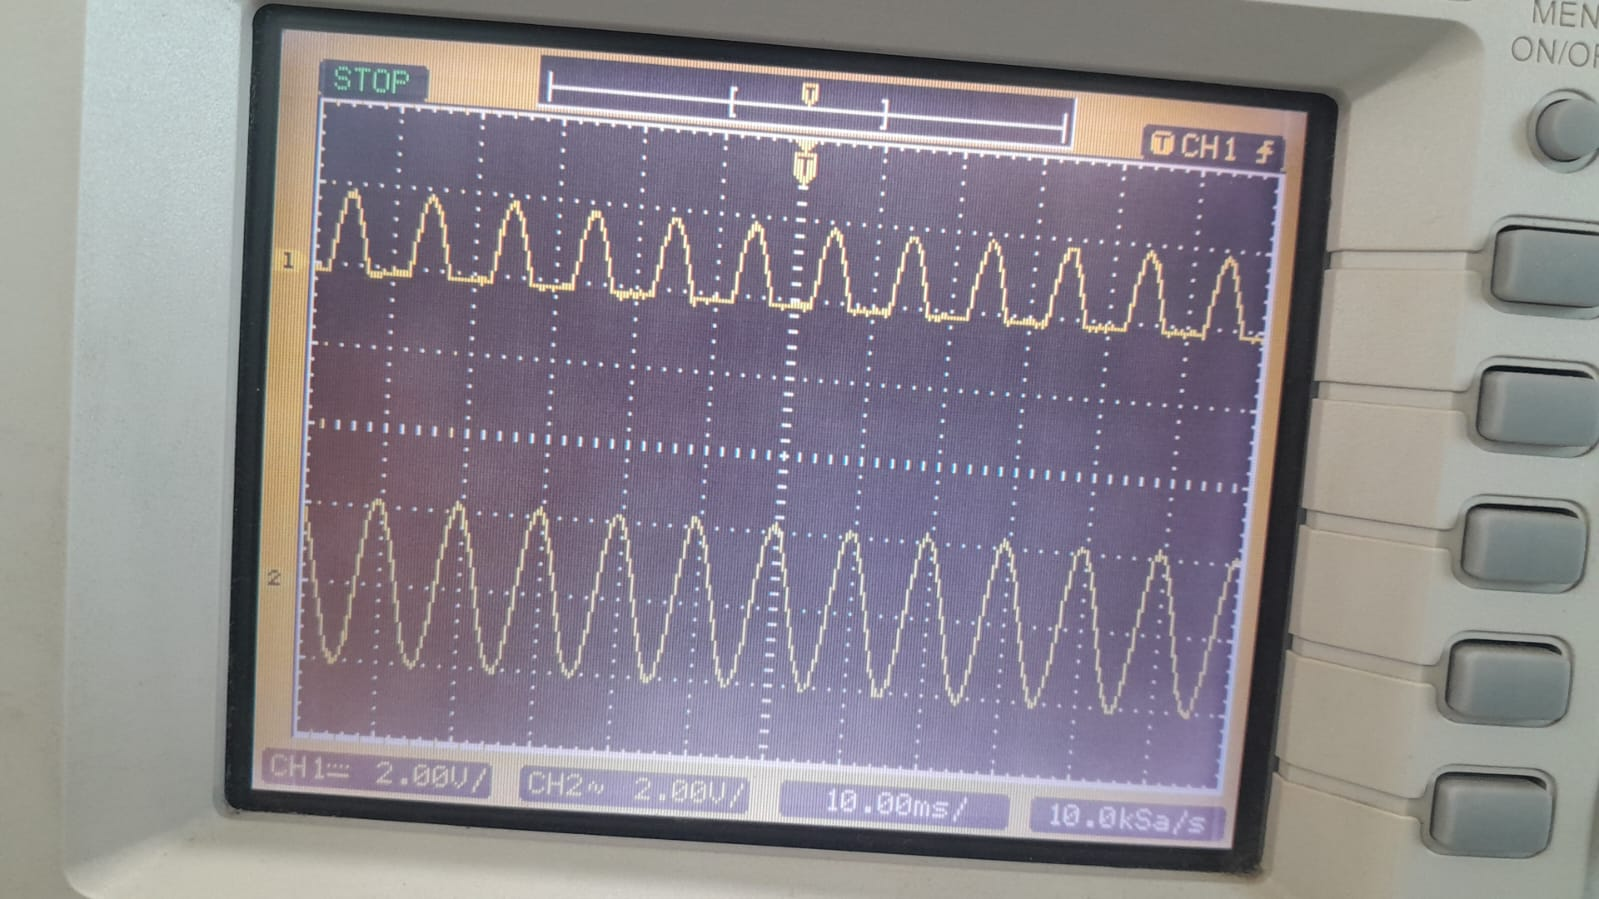
\includegraphics[width=\columnwidth]{figs/opamprect.jpg}}
  \caption{Response for resitor-diode-only circuit}
\end{figure}
\begin{figure}[H]
  {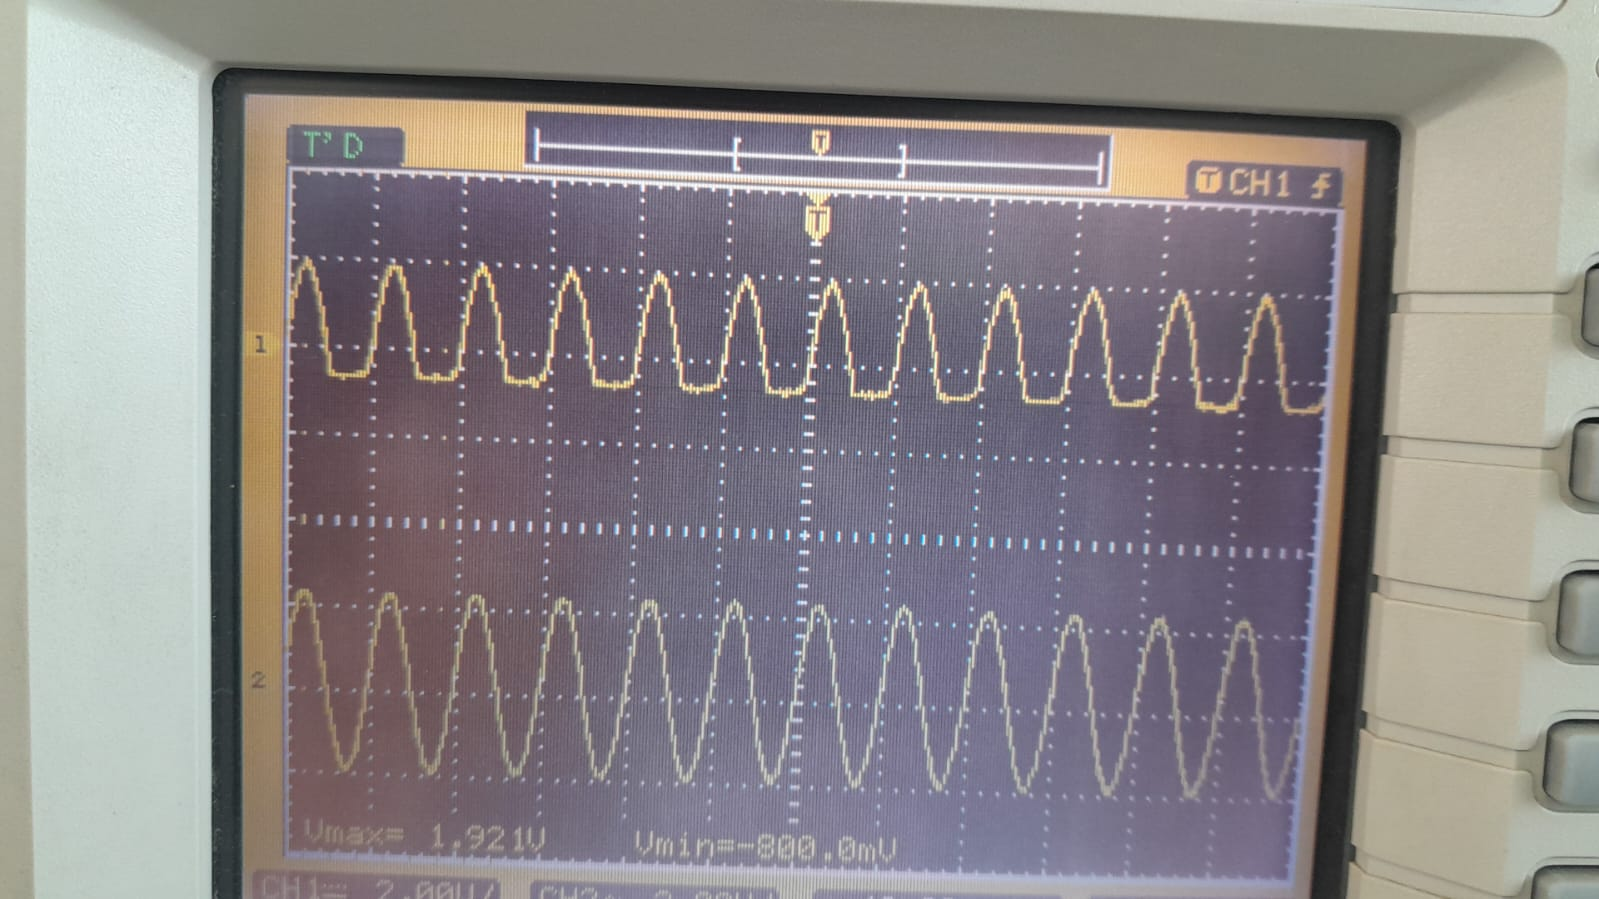
\includegraphics[width=\columnwidth]{figs/simprect.jpg}}
  \caption{Response for superdiode circuit}
\end{figure}
\end{document}
